\subsection{Network layer}

Network layer is the third layer of the \acrshort{osi} reference model. It enables interconnection of multiple networks into larger ones, and provides means for a clear and logical identification of a computer on any network.

The network layer provides functional and procedural means of transmitting variable-length data sequences from source to target by one or more networks, while being in charge of the quality of service required by the transport service. The network layer takes care of routing, data flow control, segmentation and de-segmentation, and error checking. Routers work on this layer.

On this layer, a header is added which encapsulates the  \acrfull{pdu} coming from transport layer which is a segment. The header specifies information needed for successful transmission, such as logical addresses. After adding this header, the \acrshort{pdu} is called a packet.

From a network layer perspective, the entire ``global'' network environment is partitioned into networks and subnets. Every network (subnet) has its own address that uniquely identifies it, and each computer has its own unique address in each of these networks. By combining the network address and the computer address, an address will be created that uniquely identifies the computer on any network. This address belongs to logical addresses because it depends on where your computer is located. If we transfer a computer from one network to another, its network (logical) address will change, while its physical address -- the \acrshort{mac} address -- remains the same.

Network layer tasks include:
\begin{itemize}[noitemsep]
    \item Unambiguous addressing
    \item Identifying the optimal data delivery path between the sender and the recipient
    \item Packet creation
    \item Transferring packets to the end recipient
    \item Re-composition of packets at the recipient
\end{itemize}

When the sender sends a packet to a recipient, it sends it to its predefined router for delivery. The router from the packet reads the address of the recipient, scans its subnet database, finds out to which of them the packet belongs to, and through which next nearest router the packet has to go. Once this information is obtained, it sends the packet to the specified router. This process is repeated until the packet has reached the destination network.

When sending a packet through wireless sensor network, it is often viable to use multi-hop approach; reason is that a node sending data to the base station may be far away, which means it would need to use much more energy for transmission compared to as if it was close. On top of that if there are many nodes and each of them is directly connected to a base station, a lot of interference is created when accessing the channel. Therefore, nodes must participate and forward data towards a sink; data are send to a nearest node, which forwards it further until destination is reached as it may be seen in Figure~\ref{fig:multihop}.

As already mentioned, the sender sends a packet to a predefined router and uses a predefined path for deliver. However, there is a problem with selecting the best routing path, and its solution is one of the main network layer tasks. This problem is complicated by the fact that the shortest route is not always the best. Frequently the route selection criterion is the time by which a packet can be delivered via a route; some routing algorithms determines a path by congestions between routers, while others make decisions based on average performance over a long period of time. Transfer reliability may be used as a criterion as well. The reason for the shortest path not always being the best is that there might be congestion on a path, some link may be unreliable, or it may be too power consuming to send a packet via the path. Therefore, a routing algorithm should be carefully designed to meet traffic requirements and extend lifetime of the network as much as possible, because nodes may be battery powered.

\begin{figure}
    \centering
    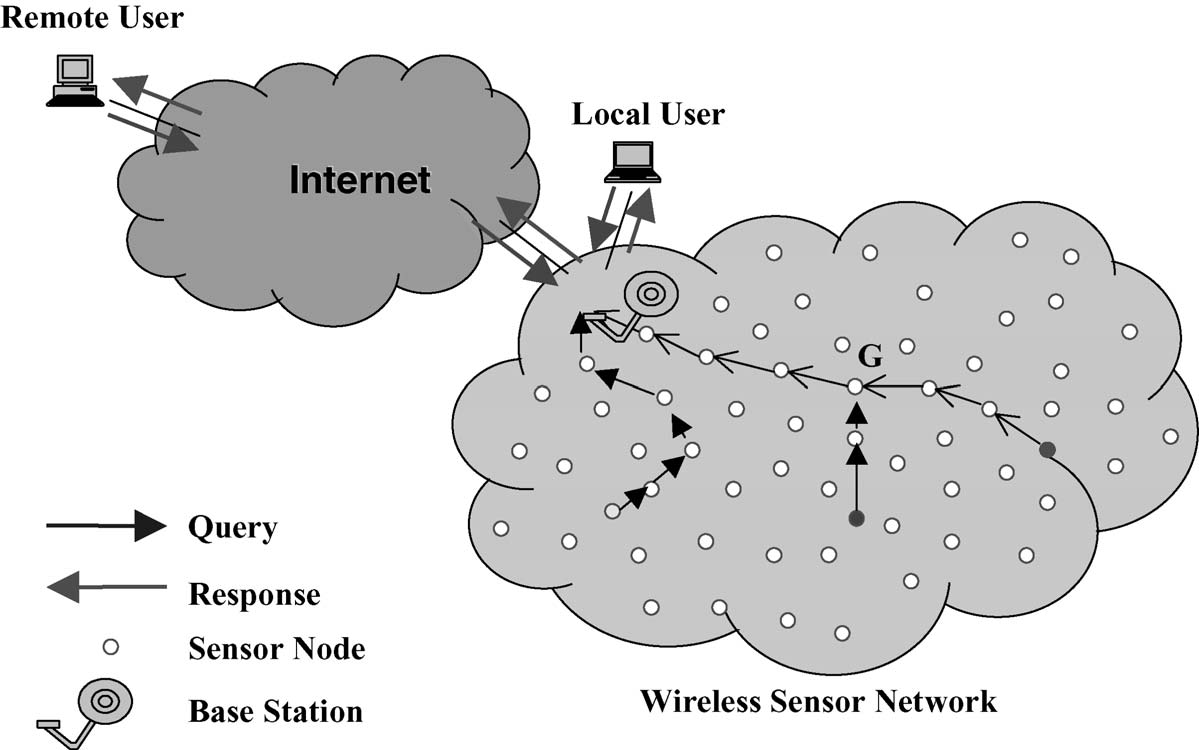
\includegraphics[width=0.8\textwidth]{00images/multihop}
    \caption{Multi-hop node communication. Taken from~\cite{Sohraby2007WirelessApplications}.}
    \label{fig:multihop}
\end{figure}

Several strategies for routing algorithms exists: proactive, reactive and hybrid strategies. Proactive strategy is based on routing tables which needs to be updated and contain global information about nodes across the network, based on them the optimal route is calculated beforehand. Such strategy is not very vital in huge \acrshort{wsn}. The reactive strategy is discovery of the best path on demand, without prior knowledge of nodes information across the network. When a path is found, reply about its hops travels all the way back to sender. The last strategy, the hybrid one is a mix of proactive and reactive strategies, where nodes are organised in clusters. Communication within cluster use proactive strategy while in between cluster the reactive one is used.

In \acrshort{wsn} networks there are several routing techniques/classes being used to achieve requirements fulfilment set by customer, e.g. power limitation, maximum delay and packet loss or resource limitation. A first class has a flat network architecture, meaning all nodes are considered to be on the same level – peers. Advantages of such architecture are possible detection of multiple paths and minimal overhead. Next class has a hierarchical network architecture, where nodes are organised into clusters with the presence of a cluster master which serves as a sink for the rest of nodes within a cluster and handles communication outside a cluster. A third class is based on data-centric approach where a node is being assigned some task and if sensed, the node sends data through the network to another node which is listening to a given attribute, until it reaches sink. The last class is based on location of node which is used for addressing. Here a location of node is relevant as a query by a source node may by specific for some area.
